%%%%%%%%%%%%%%%%
\section{Control Solution}
\begin{frame}{Control Solution}{}
    \centering
    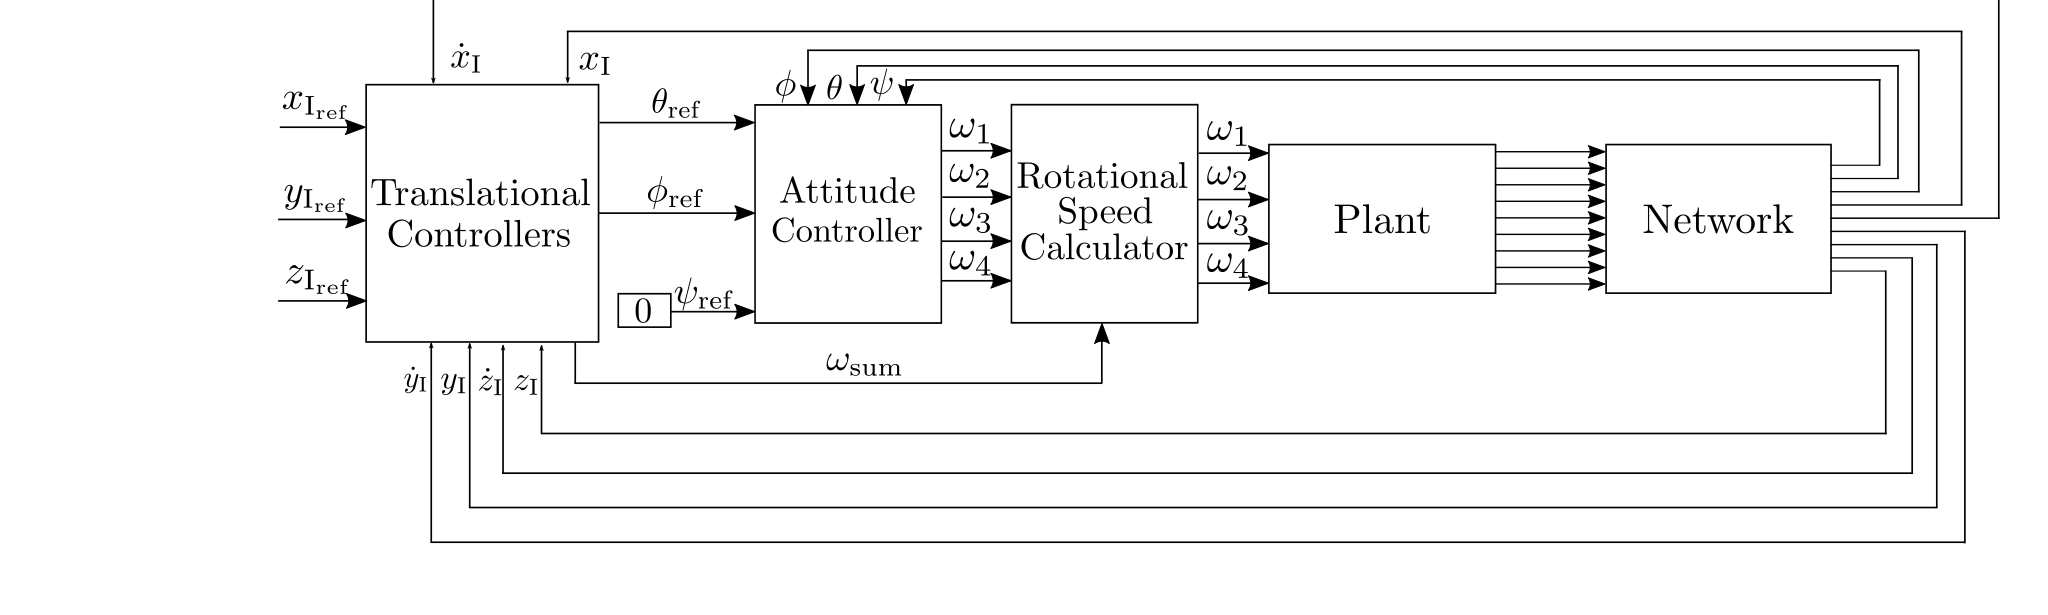
\includegraphics[scale=0.2]{figures/ControlDiagramPoster}
\end{frame}

\subsection{Attitude Controller}
\begin{frame}{Control Solution}{Attitude Controller}
    \centering
    \includegraphics[scale=0.35]{figures/AttitudeControlDiagram}    
\end{frame}

\begin{frame}{Control Solution}{Attitude Controller}
    \begin{itemize}
        \item System Representation
    \end{itemize}

%    \begin{figure}
%        \input{figures/SSBlockDiagram.tikz}
%    \end{figure}
\end{frame}


\begin{frame}{Control Solution}{Attitude Controller}
    \begin{itemize}
        \item State Feedback with Integral Control
    \end{itemize}
    
    \centering
%    \includegraphics[scale=0.25]{figures/ControllerColorDiagram}  \\
%    \vspace{1cm}
    \includegraphics[scale=0.35]{figures/DetailedControllerColorDiagram}  
    
    extended
\end{frame}

\begin{frame}{Control Solution}{Attitude Controller}
    \begin{itemize}
        \item LQR
    \end{itemize}
    \begin{flalign} 
        J &= \int_{0}^{\infty} \vec{x}^T \vec{Q} \vec{x} + \vec{u}^T \vec{R} \vec{u} \ dt \nonumber
    \end{flalign}
     \begin{itemize}
         \item Bryson's Rule
     \end{itemize}   
    \begin{flalign} 
    Q_{ii} &= \frac{1}{\text{maximum acceptable value of }[x^2_i]}\nonumber\\
    R_{ii} &= \frac{1}{\text{maximum acceptable value of }[u^2_i]}\nonumber
    \end{flalign}
    
\end{frame}

\begin{frame}{Control Solution}{Attitude Controller}
    \begin{itemize}
        \item Reduced Order Observer
    \end{itemize}
%
%
%    \begin{minipage}{\linewidth}
%        \begin{minipage}{0.49\linewidth}
%            \begin{figure}[H]
%                \includegraphics[width=1\textwidth]{figures/ObserverColorDiagram}
%            \end{figure}
%        \end{minipage}
%        \hspace{0.03\linewidth}
%        \begin{minipage}{0.49\linewidth}
            \begin{figure}[H]
                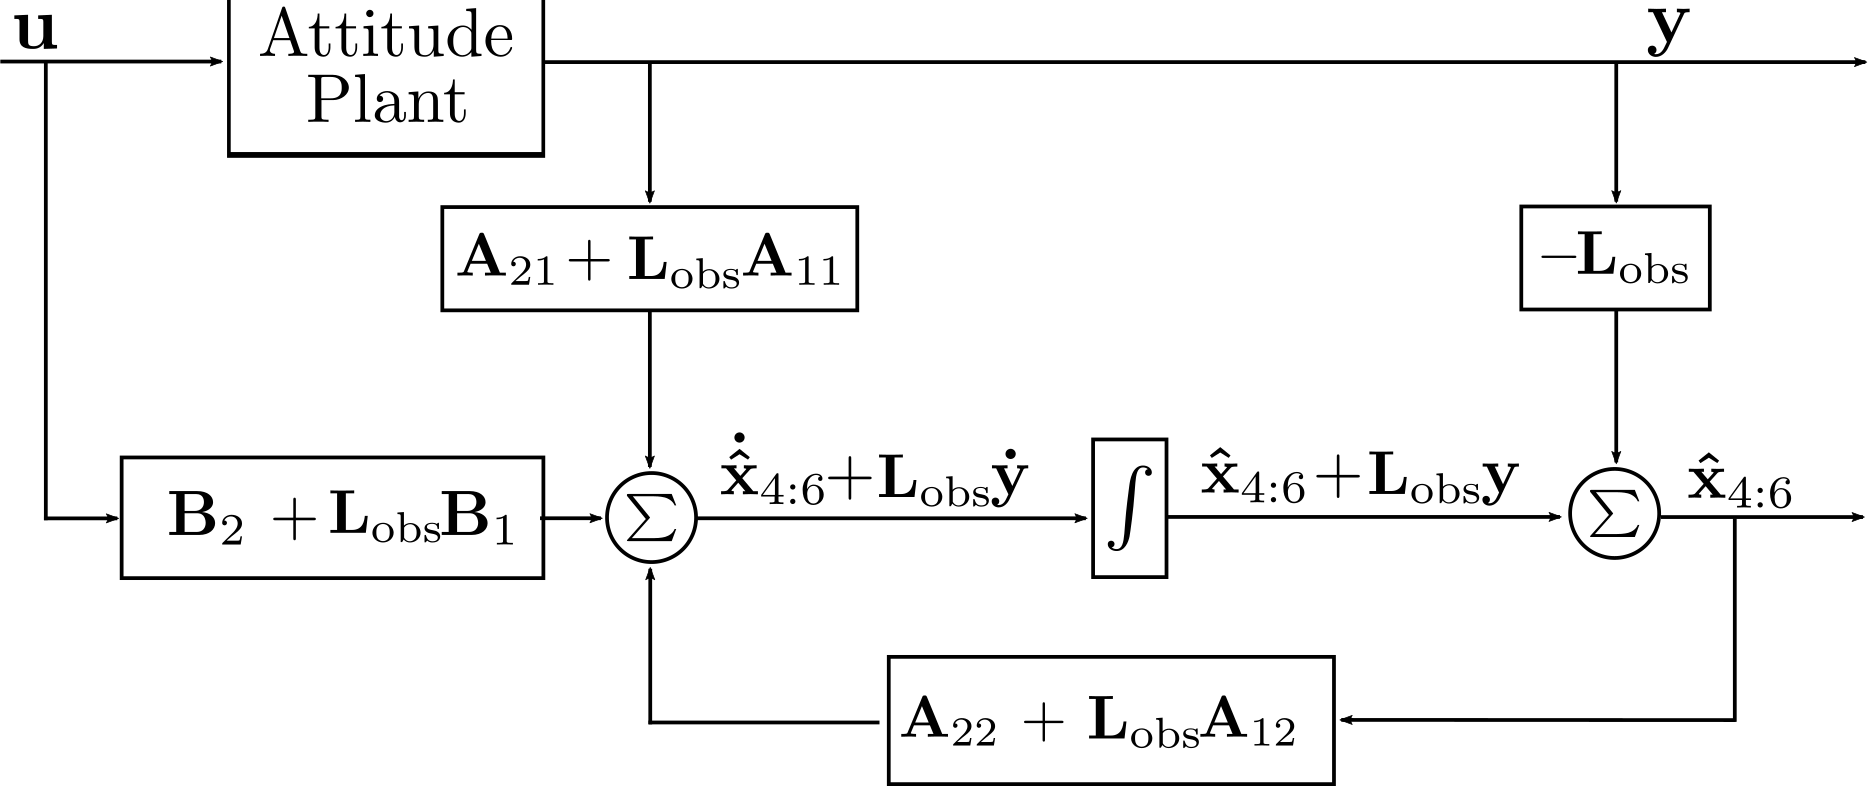
\includegraphics[width=1\textwidth]{figures/observerDiagram}
            \end{figure}                    
%        \end{minipage}
%    \end{minipage}  
    
    equation
    what are the states we estimate
   \begin{flalign}
       \vec{A_{22}} + \vec{L_{obs}}\vec{A_{12}} \nonumber
   \end{flalign}
\end{frame}

%%
% TOC
\begin{frame}{Agenda}{}
    \tableofcontents
\end{frame}

%%